\documentclass{article}
\usepackage{ctex}
\usepackage{bm}
\usepackage[colorlinks, linkcolor=blue]{hyperref}
\usepackage{geometry}
\geometry{left=3cm, right=3cm, top=3cm, bottom=3cm}
\usepackage{amsmath}
\usepackage{amsthm}
\usepackage[T1]{fontenc}
\usepackage{xcolor}
\usepackage{lmodern}
\usepackage{listings}

\newtheorem{task}{问题}

\lstset{
	numbers=left, 
	numberstyle= \small, 
	keywordstyle= \color{ blue!70},
	commentstyle= \color{red!50!green!50!blue!50}, 
	frame=shadowbox, % 阴影效果
	showstringspaces = false,
	flexiblecolumns,                % 别问为什么,加上这个
	rulesepcolor= \color{ red!20!green!20!blue!20} ,
	escapeinside=``, % 英文分号中可写入中文
	breaklines=true,
	%xleftmargin=2em,xrightmargin=2em, aboveskip=1em,
	framexleftmargin=2.7em
}

\lstdefinestyle{Fortran}{
	language        =   [90]Fortran,
	basicstyle=\small\ttfamily
}

\title{作业三:线性方程组求解}
\author{英才1701 赵鹏威 U201710152}

\begin{document}
	\maketitle
	\tableofcontents
	\newpage
	\section{引言}
	在解决实际问题的时候,常常会遇到求解线性方程组的问题,比如使用有限差分法解偏微分方程. 往往线性方程组的个数会达到上万个,因此研究高效的算法很有必要. 这次作业主要使用 Gauss 消元法、Doolittle 分解法、Gauss-Seidel 迭代法和超松弛迭代法来解线性方程组.
	
	\section{问题描述}
	\begin{task}
		分别使用 Gauss 消元法、Doolittle 分解法、超松弛 Gauss-Seidel 迭代法解以下方程组
		\[
		\bm{A}\bm{x}=
		\begin{bmatrix}
		-15 \\
		27 \\
		-23 \\
		0 \\
		-20 \\
		12 \\
		-7 \\
		10 \\
		\end{bmatrix}
		\quad
		\bm{A}=
		\begin{bmatrix}
			 31 & -13 &  0 &  0 &  0 & -10 &  0 &  0 &  0 \\
			-13 &  35 & -9 &  0 & -11 & 0 & 0 & 0 & 0 \\
			0 & -9 & 31 & -10 & 0 & 0 & 0 & 0 & 0  \\
			0 & 0 & -10 & 79 & -30 & 0 & 0 & 0 & -9  \\
			0  &0 & 0 & -30 & 57 & -7 & 0 & -5  &0 \\
			0 & 0  &0  &0 & -7 & 47 & -30 & 0  &0 \\
			0  &0  &0 & 0 & 0  &-30  &41 & 0 & 0 \\
			0& 0& 0& 0 &-5& 0& 0& 27& -2 \\
			0& 0& 0 &-9 &0& 0& 0& -2& 29 \\
		\end{bmatrix}
		\]
	\end{task}
	
	\section{程序实现}
	为了方便,使用拓展矩阵来储存线性方程组的全部信息. 由于上面提到的所有方法都不希望对角元出现 0,因此在计算之前,先对矩阵做列主元变换. 代码见 Listing \ref{pivot_exchange.f90}.
	\lstinputlisting[
	style = Fortran,
	caption     =   {\bf 列主元变换},
	label       =   {pivot_exchange.f90}
	]{./utils/snips/pivot_exchange.f90}
	
	所有的求解方法都被封装在一个叫做 linear\_eqs\_solver 的 module 里. 其中还包含了一个常数 EPSILON ,用来控制求解的精度,默认为 1e-3. 完整代码见附录.
	\subsection{Gauss 消元法}
	Gauss 消元法每次消元后矩阵大部分的值都改变了,所以 Gauss 消元法时不用上面这个列主元变换子程序,而是内置一个,即在每次消某一列之前对这一列做列主元变换. 流程图如图\ref{fig:gauss_elimination}所示. 代码见 Listing \ref{gauss_elimination.f90}.
	\begin{figure}[h!tb]
		\centering
		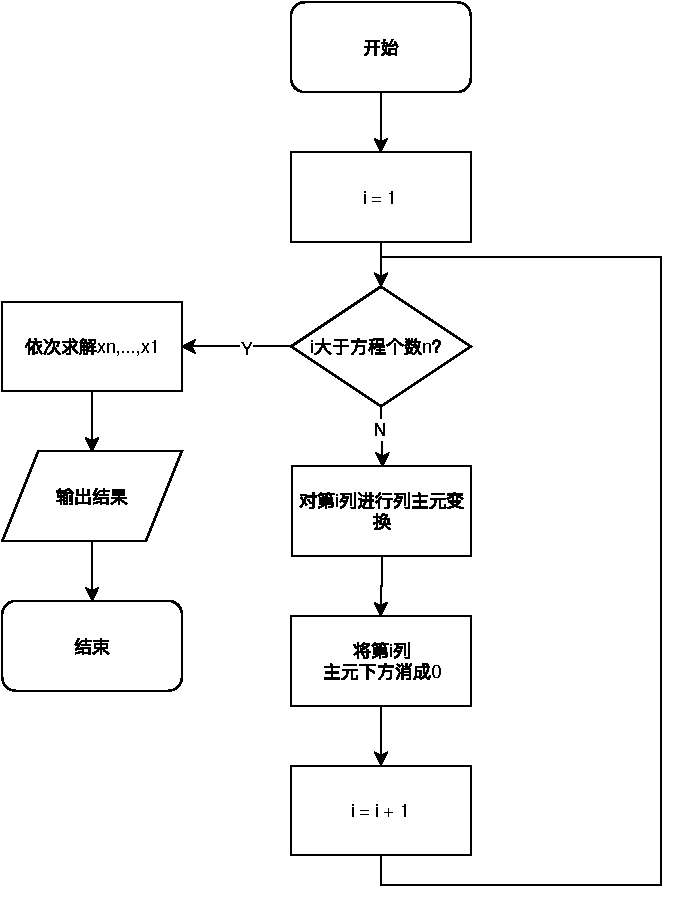
\includegraphics[width=0.5\textwidth]{./utils/gauss_elimination.pdf}
		\caption{ Gauss 消元法流程图\label{fig:gauss_elimination}}
	\end{figure}
	\lstinputlisting[
	style = Fortran,
	caption     =   {\bf Gauss 消元法},
	label       =   {gauss_elimination.f90}
	]{./utils/snips/gauss_elimination.f90}
	\subsection{Doolittle 分解法}
	Doolittle 分解法将系数矩阵分解为一个下三角矩阵和一个上三角矩阵的乘积.
	\[
	\bm{A}=\bm{L}\bm{U}
	\]
	$\bm{L}$和$\bm{U}$各分量的值可以由下式得到
	\[
	u_{k j}=a_{k j}-\sum_{r=1}^{k-1} l_{k r} u_{r j} \quad j=k,\cdots,n
	\]
	\[
	l_{i k}=\frac{a_{i k}-\sum_{r=1}^{k-1} l_{i r} u_{r k}}{u_{k k}} \quad i=k+1,\cdots,n
	\]
	方程最终的解分两步得到
	\[
	y_{i}=b_{i}-\sum_{j=1}^{i-1} I_{i j} y_{j} \quad i=1, \cdots, n
	\]
	\[
	x_{i}=\frac{y_{i}-\sum_{j=i+1}^{n} u_{i j} x_{j}}{u_{i i}} \quad i=n, \cdots, 1
	\]
	由于 Gauss 消元法和 Doolittle 分解法都是精确的算法,因此最后输出的结果误差为0(实际上不是严格的0,但是误差会比双精度浮点数最小的那个数小). 流程图见图\ref{fig:doolittle}. 代码见 Listing \ref{doolittle.f90}.
	\begin{figure}[h!tb]
		\centering
		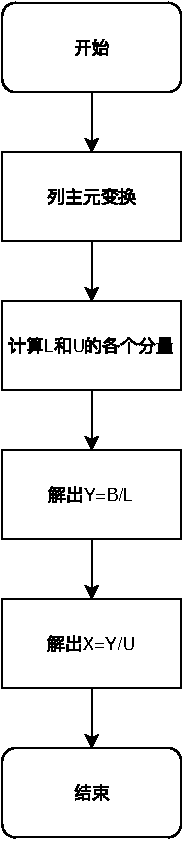
\includegraphics[width=0.18\textwidth]{./utils/doolittle.pdf}
		\caption{ Doolittle 分解法流程图\label{fig:doolittle}}
	\end{figure}
	\lstinputlisting[
	style = Fortran,
	caption     =   {\bf Doolittle 分解法},
	label       =   {doolittle.f90}
	]{./utils/snips/doolittle.f90}
	\subsection{Gauss-Seidel 迭代法}
	Gauss-Seidel 迭代法的子程序其中的参数 omega 是可选参数. 如果不输入 omega,那么默认 omega 的值为 1,即 Gauss-Seidel 迭代;如果输入 omega,若大于1则是 overrelaxation 迭代,若小于1则是 underrelaxation 迭代. 迭代初值设置为零向量. 迭代结果的误差大小取的是最后两次迭代的差值. 流程图见图\ref{fig:gs}. 代码见 Listing \ref{gauss_seidel_iteration.f90}.
	\begin{figure}[h!tb]
		\centering
		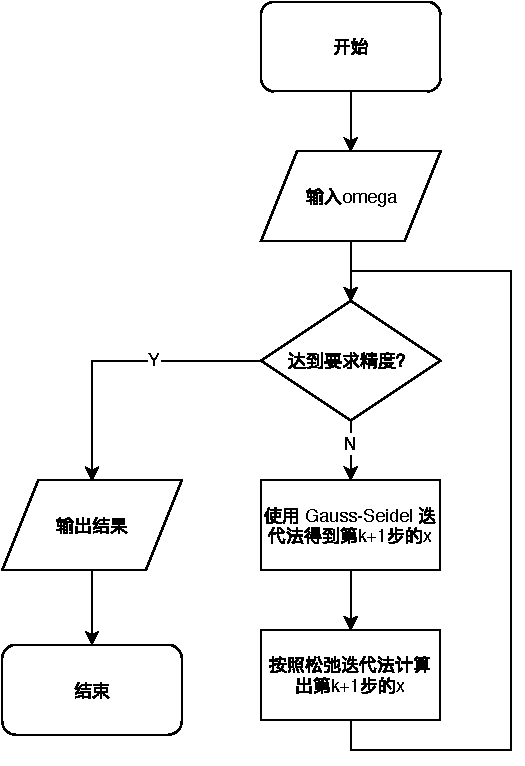
\includegraphics[width=0.5\textwidth]{./utils/gs.pdf}
		\caption{ 使用松弛迭代的Gauss-Seidel 迭代法流程图\label{fig:gs}}
	\end{figure}
	\lstinputlisting[
	style = Fortran,
	caption     =   {\bf Gauss-Seidel 迭代法},
	label       =   {gauss_seidel_iteration.f90}
	]{./utils/snips/gauss_seidel_iteration.f90}
	
	\section{运行时结果}
	\subsection{Gauss 消元法}
	Gauss 消元法的运行时结果如图\ref{fig:rtr_gauss}所示. 
	\begin{figure}[h!tb]
		\centering
		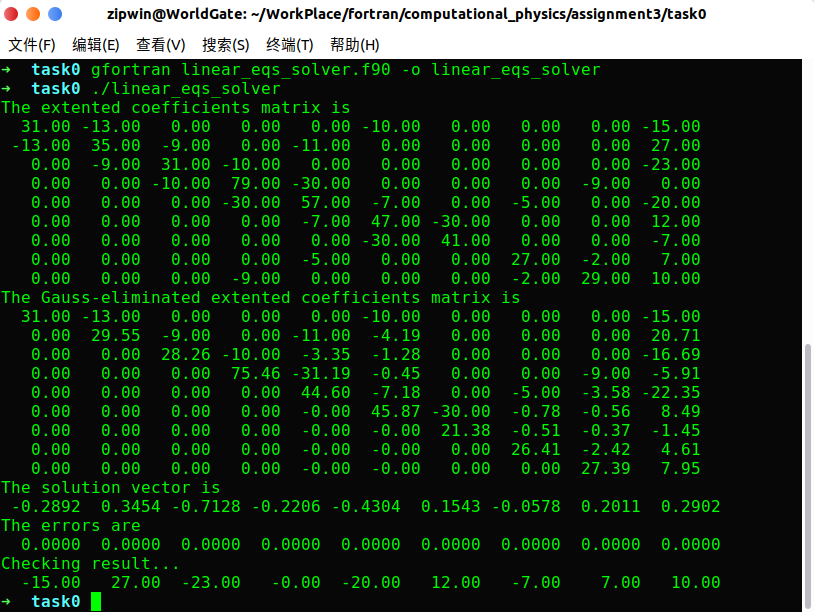
\includegraphics[width=0.7\textwidth]{./utils/rtr_gauss.png}
		\caption{Gauss 消元法\label{fig:rtr_gauss}}
	\end{figure}
	得到的结果为
	\[
	\mathrm{x}=
	\begin{bmatrix}
	-0.2892 & 0.3454 & -0.7128 & -0.2206 & -0.4304 & 0.1543 & -0.0578 & 0.2011 & 0.2982
	\end{bmatrix}^T
	\]
	命令行中 Checking results... 的下一行是将数值结果代回原方程得到的值,可见完全满足方程组(也就是和拓展矩阵的最后一列相等)
	\subsection{Doolittle 分解法}
	Doolittle 分解法的运行时结果如图\ref{fig:rtr_doolittle},结果与 Gauss 消元法完全一致.
	\begin{figure}[h!tb]
		\centering
		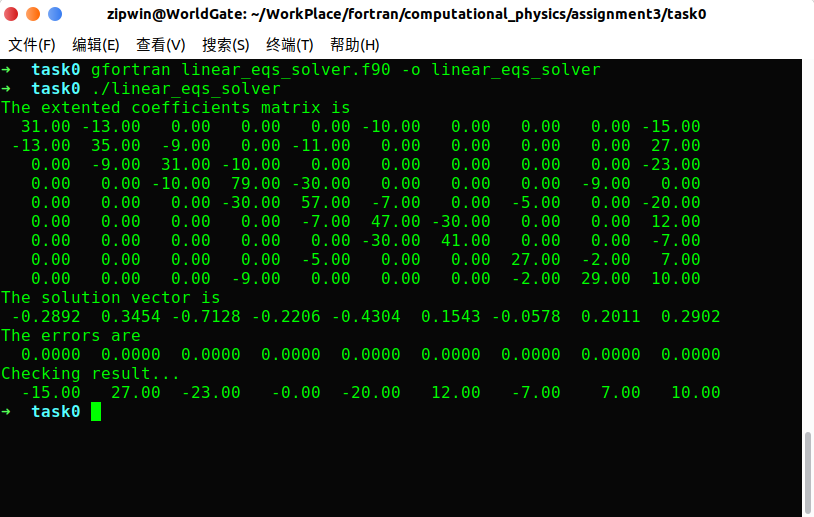
\includegraphics[width=0.7\textwidth]{./utils/rtr_doolittle.png}
		\caption{Doolittle 分解法\label{fig:rtr_doolittle}}
	\end{figure}
	\subsection{超松弛 Gauss-Seidel 迭代法}
	设置 omega 为 1.5,使用 Gauss-Seidel 迭代法的运行时结果如图\ref{fig:rtr_overgs}所示.
	\begin{figure}[h!tb]
		\centering
		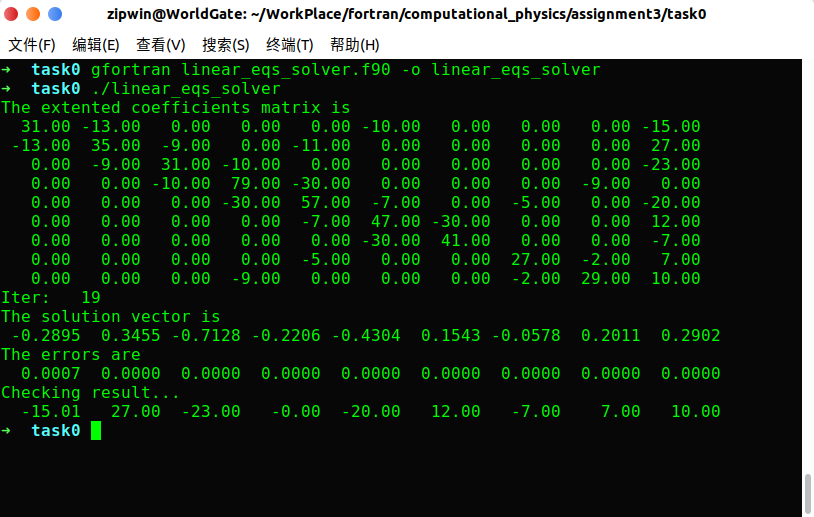
\includegraphics[width=0.7\textwidth]{./utils/rtr_overgs.png}
		\caption{超松弛 Gauss-Seidel 迭代法\label{fig:rtr_overgs}}
	\end{figure}
	得到的结果为
	\[
	\mathrm{x}=
	\begin{bmatrix}
	-0.2895 & 0.3455 & -0.7128 & -0.2206 & -0.4304 & 0.1543 & -0.0578 & 0.2011 & 0.2982
	\end{bmatrix}^T
	\]
	除第一个数有0.0007的误差外,其他的都没有误差. 达到需求的精度迭代了19次. 代回方程组检验发现,第一个方程有0.01的偏差.
	
	\section*{附录}
	代码可在\url{https://github.com/ZipWin/computational_physics/tree/master/assignments/assignment3}找到.
	\lstinputlisting[
	style = Fortran,
	caption     =   {\bf linear\_eqs\_solver.f90},
	label       =   {linear_eqs_solver.f90}
	]{./utils/linear_eqs_solver.f90}
	
	
\end{document}